% Section 2: Assumptions, Justifications, and System Boundary
% 假设、合理性证明与系统边界

\section{Assumptions, Justifications, and System Boundary}
\label{sec:assumptions}

%=== 2.1 核心假设与合理性证明 ===
\subsection{Core Assumptions and Justifications}
\label{subsec:assumptions}

% 【E题要求】假设必须与可持续性评估相关,每条假设需有独立的合理性证明

To establish a tractable yet meaningful sustainability assessment framework, we make the following assumptions. Each assumption is paired with its rationale and potential implications if violated.

\begin{enumerate}[label=\textbf{A\arabic*.}, leftmargin=2.5em, itemsep=0.8em]
    
    \item \textbf{System Stationarity Assumption.}
    The fundamental relationships among environmental, economic, and social variables remain structurally stable within the modeling horizon.
    
    \textit{Justification:} While absolute values may change, the direction and approximate magnitude of causal relationships (e.g., emissions-temperature, investment-job creation) are supported by established scientific consensus over decadal timescales~\cite{ipcc2023synthesis}.
    
    \textit{If violated:} Structural breaks (e.g., technological disruptions, regime changes) would require model re-calibration or scenario branching.
    
    \item \textbf{Data Representativeness Assumption.}
    Available datasets adequately capture the spatial and temporal heterogeneity of the system under study.
    
    \textit{Justification:} We rely on authoritative sources including \TODO{e.g., IPCC, World Bank, national statistical bureaus} with documented quality control procedures.
    
    \textit{If violated:} Systematic data gaps may bias indicator scores; we address this through sensitivity analysis in Section~\ref{sec:sensitivity}.
    
    \item \textbf{Stakeholder Rationality Assumption.}
    Stakeholders behave in a bounded-rational manner, responding to incentives and information within their cognitive and resource constraints.
    
    \textit{Justification:} This is a standard assumption in policy analysis and mechanism design, enabling scenario modeling of policy responses.
    
    \textit{If violated:} Irrational or adversarial behavior may undermine policy effectiveness; robust scenario design helps mitigate this risk.
    
    \item \textbf{Linear Aggregation Assumption (for MCDA).}
    Sustainability indicators can be meaningfully aggregated through weighted linear combination within each pillar.
    
    \textit{Justification:} While strong non-linearities exist at extreme values, linear aggregation provides transparency and is widely adopted in sustainability indices (e.g., SDG Index, EPI).
    
    \textit{If violated:} We complement MCDA with trade-off frontier analysis that explicitly preserves multi-dimensional structure.
    
    \item \textbf{Policy Implementation Assumption.}
    Proposed policies, once adopted, are implemented with the intended intensity and coverage.
    
    \textit{Justification:} This enables clean scenario comparisons. Real-world implementation gaps are acknowledged in our Discussion section.
    
    \textit{If violated:} Actual outcomes may fall short of modeled projections; adaptive management recommendations account for this.
    
    \item \textbf{Discounting Assumption.}
    Future costs and benefits are discounted at a constant rate $r$ = \TODO{e.g., 3\%} for economic valuation.
    
    \textit{Justification:} This rate reflects social time preference and opportunity cost of capital, following \TODO{e.g., Stern Review, EPA guidelines}.
    
    \textit{If violated:} Sensitivity to discount rate is examined in Section~\ref{sec:sensitivity}.
    
\end{enumerate}

%=== 2.2 系统边界定义 ===
\subsection{System Boundary Definition}
\label{subsec:boundary}

% 【E题核心】系统边界必须明确界定,避免无边界扩张

A critical step in sustainability assessment is explicitly defining what is \textit{inside} versus \textit{outside} the analytical boundary. Our system boundary is specified along four dimensions:

\subsubsection{Spatial Boundary}
\begin{itemize}[itemsep=0.2em]
    \item \textbf{Primary Scope:} \TODO{e.g., Regional watershed, national territory, urban metropolitan area}
    \item \textbf{Cross-Boundary Flows Considered:} \TODO{e.g., Transboundary pollution, trade-embedded emissions, migration}
    \item \textbf{Excluded:} \TODO{e.g., Global feedback effects beyond direct cross-boundary flows}
\end{itemize}

\subsubsection{Temporal Boundary}
\begin{itemize}[itemsep=0.2em]
    \item \textbf{Historical Data Window:} \TODO{e.g., 2000--2024 for model calibration}
    \item \textbf{Projection Horizon:} \TODO{e.g., 2025--2050 for scenario analysis}
    \item \textbf{Time Step:} \TODO{e.g., Annual for system dynamics, 5-year intervals for policy evaluation}
\end{itemize}

\subsubsection{Sectoral Boundary}
\begin{itemize}[itemsep=0.2em]
    \item \textbf{Included Sectors:} \TODO{e.g., Energy, agriculture, transportation, manufacturing}
    \item \textbf{Excluded Sectors:} \TODO{e.g., Defense, international trade beyond direct emissions}
\end{itemize}

\subsubsection{Impact Categories}
\begin{itemize}[itemsep=0.2em]
    \item \textbf{Environmental:} \TODO{e.g., GHG emissions, water quality, land use change, biodiversity}
    \item \textbf{Economic:} \TODO{e.g., GDP, employment, investment, operating costs}
    \item \textbf{Social:} \TODO{e.g., Public health, equity (Gini coefficient), education access, community resilience}
\end{itemize}

% 系统边界图示
\begin{figure}[H]
    \centering
    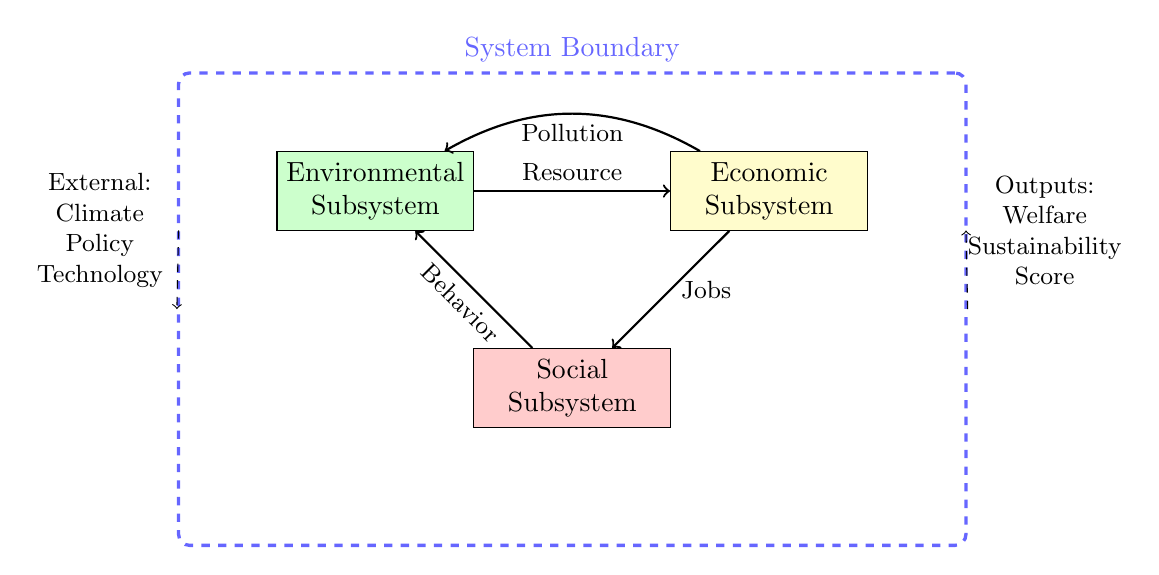
\begin{tikzpicture}[
        node distance=1cm,
        box/.style={rectangle, draw, minimum width=2.5cm, minimum height=1cm, align=center},
        boundary/.style={rectangle, draw=blue!60, very thick, dashed, rounded corners}
    ]
        % 系统边界框
        \node[boundary, minimum width=10cm, minimum height=6cm, label={[blue!60]above:System Boundary}] (sys) {};
        
        % 内部组件
        \node[box, fill=green!20] at (-2.5, 1.5) (env) {Environmental\\Subsystem};
        \node[box, fill=yellow!20] at (2.5, 1.5) (econ) {Economic\\Subsystem};
        \node[box, fill=red!20] at (0, -1) (social) {Social\\Subsystem};
        
        % 交互箭头
        \draw[->, thick] (env) -- node[above, sloped, font=\small] {Resource} (econ);
        \draw[->, thick] (econ) -- node[right, font=\small] {Jobs} (social);
        \draw[->, thick] (social) -- node[below, sloped, font=\small] {Behavior} (env);
        \draw[->, thick] (econ) to[bend right=30] node[below, font=\small] {Pollution} (env);
        
        % 外部因素
        \node[align=center, font=\small] at (-6, 1) {External:\\Climate\\Policy\\Technology};
        \draw[->, dashed] (-5, 1) -- (sys.west);
        
        \node[align=center, font=\small] at (6, 1) {Outputs:\\Welfare\\Sustainability\\Score};
        \draw[->, dashed] (sys.east) -- (5, 1);
    \end{tikzpicture}
    \caption{System boundary diagram showing included subsystems and their interactions.}
    \label{fig:boundary}
\end{figure}

%=== 2.3 数据来源说明 ===
\subsection{Data Sources}
\label{subsec:data_sources}

% 【数据透明性】O奖论文需明确数据来源

Our analysis draws on the following data sources:

\begin{table}[H]
    \centering
    \caption{Summary of Data Sources}
    \label{tab:data_sources}
    \begin{tabularx}{\textwidth}{l l X l}
        \toprule
        \textbf{Category} & \textbf{Source} & \textbf{Variables} & \textbf{Period} \\
        \midrule
        Environmental & \TODO{e.g., IPCC, EPA} & \TODO{e.g., GHG emissions, temperature} & \TODO{years} \\
        Economic & \TODO{e.g., World Bank, OECD} & \TODO{e.g., GDP, investment, employment} & \TODO{years} \\
        Social & \TODO{e.g., UN, census data} & \TODO{e.g., Population, health, education} & \TODO{years} \\
        Geospatial & \TODO{e.g., NASA, USGS} & \TODO{e.g., Land use, satellite imagery} & \TODO{years} \\
        \bottomrule
    \end{tabularx}
\end{table}
